\documentclass[11pt, letter, margin = 2 in]{article}

\usepackage[style = authoryear, autocite=inline, doi=false,isbn=false,url=false]{biblatex}
\usepackage[colorlinks, citecolor = red]{hyperref}
\usepackage[long, nodayofweek]{datetime}
\usepackage[]{booktabs}
\usepackage{graphicx}
\usepackage{amsmath}

\usepackage[sf,pagestyles]{titlesec} % make section headings \sffamily
% make headers \sffamily
\newpagestyle{main}[\sffamily]{
    \sethead{\thepage}{}{\sectiontitle}
    }
\pagestyle{main}
\usepackage{titling}
% make titling elements \sffamily
\pretitle{\begin{center}\sffamily\LARGE}
\preauthor{\begin{center}
            \large\sffamily \lineskip 0.5em%
            \begin{tabular}[t]{c}}
\predate{\begin{center}\sffamily\large}
\usepackage{abstract}
% make abstract title \sffamily
\renewcommand\abstractnamefont{\sffamily}
\usepackage{caption} 
\captionsetup{font=sf, labelfont = bf}

\begin{document}
\author{Andy Eggers\thanks{Nuffield College and Department of Politics and International Relations, University of Oxford, United Kingdom. \texttt{aeggers@nuffield.ox.ac.uk}}
\and
Tobias Nowacki\thanks{Department of Political Science, Stanford University, CA, United States. \texttt{tnowacki@stanford.edu}}}
\date{\today}
\title{Regression Model Idea}

\maketitle

\section{Introduction}

This memo maps out the idea of using regression models to capture some of the more complex interplays between model parameters. The goal of this approach is to enable us to offer straightforward summaries, such as: "the more the vote share for A increases, the more does a probability of a strategic vote being optimal increase."

\section{Concept}

For the purpose of this memo, a toy model approach will suffice. Let's simulate a distribution of expected ballot profiles from the following hyperprior:

\begin{align}
40 \times (.3, \ .13, \ .185, \ .185, \ .03, \ .17)
\end{align}

The simulation yields 1,000 draws from this Dirichlet hyperprior. For each of these draws, I check whether, at $s = 85$, either ABC or ACB voters (with utility function (1, $\beta$ = 0.5, 0)) have an incentive to vote strategically (that is, $\tau > 0$). Going forward, we can be more precise with our outcome of interest here, and model parameter dynamics for the outcome of $ABC$ voters, for example, putting their second choice as first on the ballot. 

\section{Modelling}

Unsure how to do that yet -- many different options. This should be guided by theory.

\begin{figure}[!htb]
	\centering
	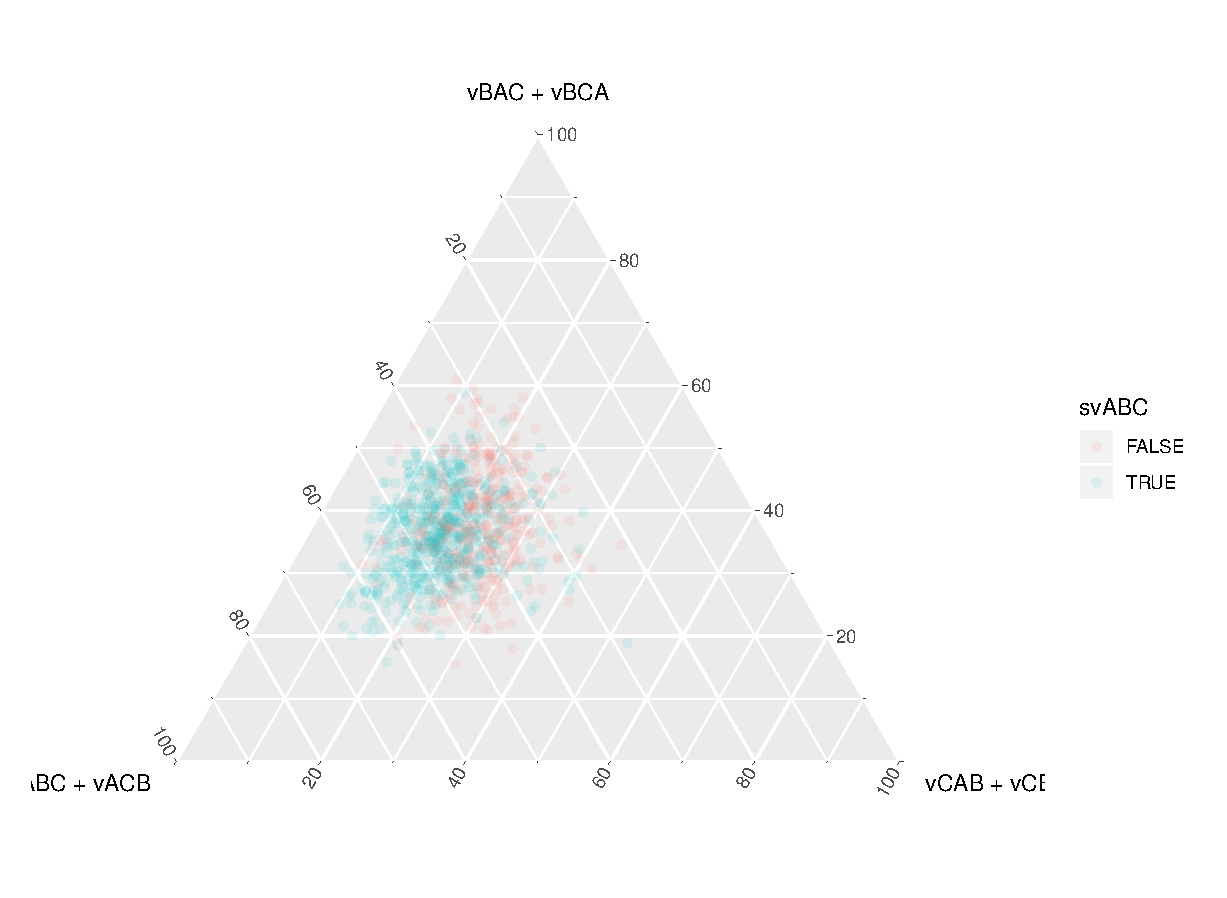
\includegraphics[width = 0.5 \textwidth]{../output/figures/regression/abc.pdf}
	\caption{Strategic Voting optimal for ABC Voter?}
	\label{fig:figure1}
\end{figure}

\begin{figure}[!htb]
	\centering
	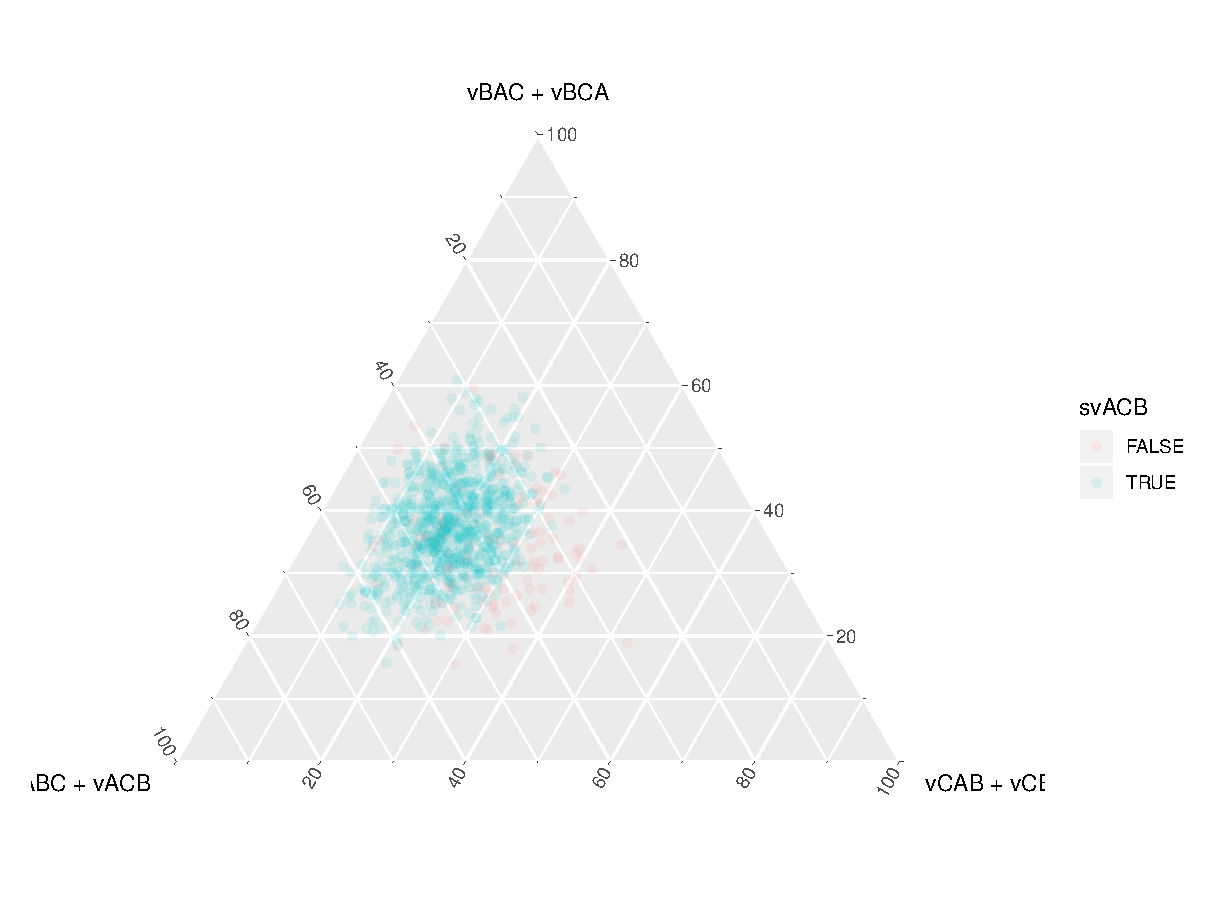
\includegraphics[width = 0.5 \textwidth]{../output/figures/regression/acb.pdf}
	\caption{Strategic Voting optimal for ACB Voter?}
	\label{fig:figure1}
\end{figure}

Table~\ref{tab:regmods} reports the results of the basic, experimental model. What seems to matter is, for ABC voters, that both $A$ and $B$ are strong (i.e., we're far to the left of the ternary diagram). For ACB voters, on the other hand, there seems to be no interaction effect: both strong A and strong B situations are conducive to strategic voting. Another observation is that strategic voting is more likely for ABC voters in single-peaked cases (when $m_{AB}$ is high); this is not true for ACB voters (Why?).

Potential problem here is that the results are very volatile and highly sensitive to the parametrisation of the initial hyperprior. Perhaps best to cover the entire simplex instead?

\begin{table}[!htbp] \centering 
  \caption{Regression results} 
  \label{tab:regmods} 
\begin{tabular}{@{\extracolsep{5pt}}lcc} 
\\[-1.8ex]\hline 
\hline \\[-1.8ex] 
 & \multicolumn{2}{c}{\textit{Dependent variable:}} \\ 
\cline{2-3} 
\\[-1.8ex] & \multicolumn{2}{c}{NA} \\ 
\\[-1.8ex] & (1) & (2)\\ 
\hline \\[-1.8ex] 
 I(vABC + vACB) & $-$0.242 & 1.650$^{***}$ \\ 
  & (0.717) & (0.438) \\ 
  & & \\ 
 I(vBAC + vBCA) & $-$2.655$^{***}$ & 1.572$^{***}$ \\ 
  & (0.834) & (0.510) \\ 
  & & \\ 
 I((vABC + vACB) \textasteriskcentered  (vBAC + vBCA)) & 9.780$^{***}$ & 0.528 \\ 
  & (1.953) & (1.193) \\ 
  & & \\ 
 $m_{AB}$ & 0.432$^{***}$ & $-$0.101 \\ 
  & (0.126) & (0.077) \\ 
  & & \\ 
 $m_{CB}$ & 1.088$^{***}$ & 1.073$^{***}$ \\ 
  & (0.111) & (0.068) \\ 
  & & \\ 
 Constant & $-$1.055$^{***}$ & $-$1.318$^{***}$ \\ 
  & (0.354) & (0.216) \\ 
  & & \\ 
\hline \\[-1.8ex] 
Observations & 1,000 & 1,000 \\ 
R$^{2}$ & 0.258 & 0.319 \\ 
\hline 
\hline \\[-1.8ex] 
\textit{Note:}  & \multicolumn{2}{r}{$^{*}$p$<$0.1; $^{**}$p$<$0.05; $^{***}$p$<$0.01} \\ 
\end{tabular} 
\end{table} 



\end{document}